\chapter{Supplementary material for \autoref{chap:rys}}

\section{Synteny analysis of genomic surroundings of \textit{D. rerio} npat}
\autoref{synteny} displays the output of the Synteny Database tool \cite{Catchen2009} for the genomic region hosting npat on \textit{D. rerio} chromosome 15. On the scaffold of \textit{H. sapiens} chromosome 11, NPAT occurs upstream of the highlighted duplication cluster bracketed by ARCN1 and MIZF. Zebrafish npat is located in the midst of this rearranged, duplicated cluster, but does not appear to have been duplicated itself; at least if it was, no paralogue can be found by syntenic or similarity analysis.


\begin{sidewaysfigure}[!h]
    \makebox[\textwidth][c]{\includegraphics[width=1.2\textwidth]{rys/synteny2.png}}    
    \caption{{\bf Synteny Database output for the syntenic region containing \textit{D. rerio} npat}}
    Dre\#: \textit{Danio rerio chromosome \#}
    Hsa\#: \textit{Homo sapiens chromosome \#}

    The relative position of the displayed genomic neighbourhoods on their chromosome scaffolds is displayed inset, top right. \textit{D. rerio} npat is highlighted with a red square, visible on the right of the selected Dre15 region, annotated ``im:6901964''. \textit{H. sapiens} NPAT is highlighted similarly on the left of Hsa11. landmarks of the duplication and rearrangement event that brackets the position of npat on Dre15 are highlighted with red lines.
    \label{synteny}
\end{sidewaysfigure}

\section{10dpf \textit{rys} RPCs are mitotic}

\begin{figure}[!h]
    \makebox[\textwidth][c]{\includegraphics[width=1.\textwidth]{rys/cmzfailure.png}}    
    \caption{{\bf Rys CMZ RPCs are mitotic at 10dpf}} MIP 14\si{\micro\metre} coronal cryosections through representative sib (left panels) and \textit{rys} eyes at 10dpf, 7 days after an 8hr BrdU pulse at 3dpf. Note that few labelled \textit{rys} cells have entered the specified retinal layers.
    \label{rysmitosis}
\end{figure}


\section{The fate of \textit{rys} RPCs is microglial phagocytosis}

\begin{figure}[!h]
    \makebox[\textwidth][c]{\includegraphics[width=1.\textwidth]{rys/rys_4c4.png}}    
    \caption{{\bf 4C4-positive microglia engulf \textit{rys} mutant RPCs}} 
    \label{phagocytosis}
\end{figure}

\section{PWM sources detected in the combined sib and rys differential position set}

\begin{figure}[!h]
    \makebox[\textwidth][c]{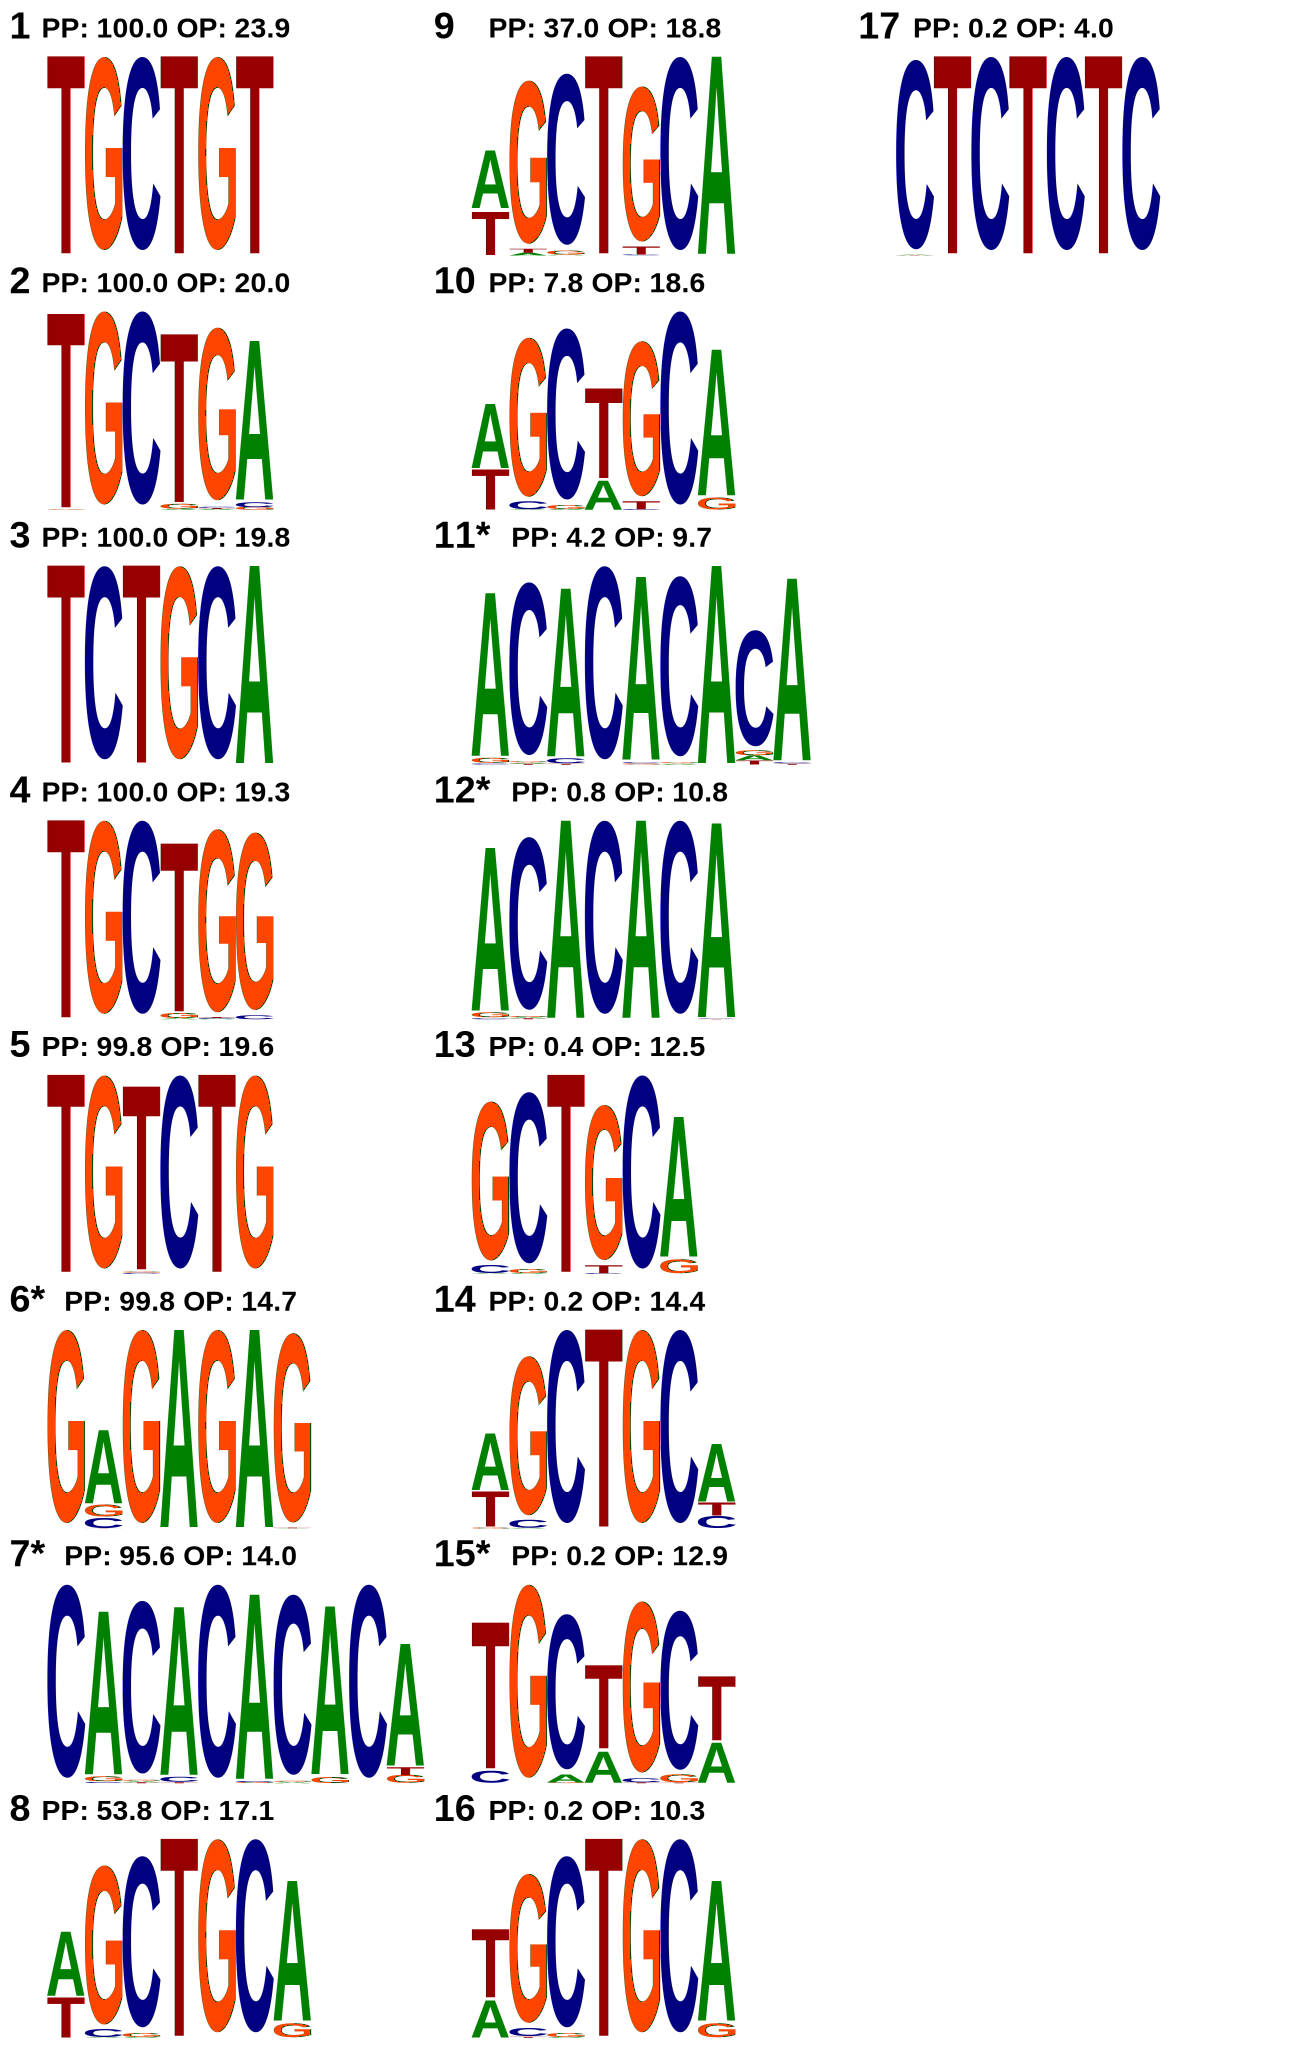
\includegraphics[width=.75\textwidth]{rys/combined_e_srcs.png}}    
    \caption{{\bf PWM sources detected in combined differential sources.}}
    Counts of positions found in sib but not rys (red bars, represented as negative numbers, as these are `lost' in rys) and those found in rys but not sib (blue bars, `gained'). The magnitude of the difference between the counts is represented with a yellow bar.
    \label{combinedmotifs}
\end{figure}
